\documentclass[xcolor=x11names,compress,professionalfonts, aspectratio=169]{beamer}

%% General packages %%%%%%%%%%%%%%%%%%%%%%%%%%%%%%%%%%
\usepackage[utf8]{inputenc}
\usepackage{graphicx}
\usepackage{tikz}
\tikzset{% change default arrow tips
    >=latex
}
\usepackage{ifthen}

\usepackage{amsmath}
\usepackage{nicefrac}

\usepackage{color}

% compile child documents using this preamble
\usepackage{subfiles}

% compile child files with separate preambles, and include them in the document
\usepackage{standalone}

%%%%%%%%%%%%%%%%%%%%%%%%%%%%%%%%%%%%%%%%%%%%%%%%%%%%%%

\makeatletter
\setbeamertemplate{footline}
{
    \leavevmode%
    \hbox{%
        \begin{beamercolorbox}[wd=.333333\paperwidth,ht=2.25ex,dp=1ex,center]{author in head/foot}%
            \usebeamerfont{author in head/foot}\insertshortauthor
        \end{beamercolorbox}%
                \begin{beamercolorbox}[wd=.333333\paperwidth,ht=2.25ex,dp=1ex,center]{title in head/foot}%
            \usebeamerfont{title in head/foot}\insertshorttitle
        \end{beamercolorbox}%
        \begin{beamercolorbox}[wd=.333333\paperwidth,ht=2.25ex,dp=1ex,right]{date in head/foot}%
            \usebeamerfont{date in head/foot}\insertshortdate{}\hspace*{2em}
            \insertframenumber{} / \inserttotalframenumber\hspace*{2ex} 
        \end{beamercolorbox}}%
        \vskip0pt%
    }
    \makeatother


%% Beamer Layout %%%%%%%%%%%%%%%%%%%%%%%%%%%%%%%%%%
\useoutertheme[subsection=false,shadow]{miniframes}
\useinnertheme{rectangles}

\setbeamertemplate{navigation symbols}{}%remove navigation symbols

\author{Nicolas Macé}

\newcommand{\btVFill}{\vskip0pt plus 1filll}%place an element at the bottom of the page

\usepackage{libertine}
\usepackage[T1]{fontenc}

\setbeamerfont{title like}{shape=\scshape}
\setbeamerfont{frametitle}{shape=\scshape}

\setbeamercolor*{lower separation line head}{bg=DeepSkyBlue4} 
\setbeamercolor*{normal text}{fg=black,bg=white} 
\setbeamercolor*{alerted text}{fg=red} 
\setbeamercolor*{example text}{fg=black} 
\setbeamercolor*{structure}{fg=black} 
 
\setbeamercolor*{palette tertiary}{fg=black,bg=black!10} 
\setbeamercolor*{palette quaternary}{fg=black,bg=black!10} 

\renewcommand{\(}{\begin{columns}}
\renewcommand{\)}{\end{columns}}
\newcommand{\<}[1]{\begin{column}{#1}}
\renewcommand{\>}{\end{column}}

\definecolor{BostonBlue}{HTML}{00688B}
\definecolor{Complementary}{HTML}{8B2300}

% letters A and B appearing in the qp chains
\newcommand{\A}{\textcolor{BostonBlue}{A}}
\newcommand{\B}{\textcolor{Complementary}{B}}

\renewcommand{\ss}[1]{\scriptsize{\text{#1}}}
%%%%%%%%%%%%%%%%%%%%%%%%%%%%%%%%%%%%%%%%%%%%%%%%%%

\usepackage{braket}
% compile child documents using this preamble
\usepackage{subfiles}

%%%My Math

\newcommand{\pd}[2]{\frac{\displaystyle \partial #1}{\displaystyle\partial #2}} % for partial derivatives
\renewcommand{\d}[1]{\mathrm{d}#1}

\begin{document}

\section{2D models: the ``grown-up example''}
\subsection{Dummy}

\begin{frame}{2D tilings}
We consider the Penrose and the Ammann-Beenker tilings.
\begin{columns}
\begin{column}{5cm}
{\centering
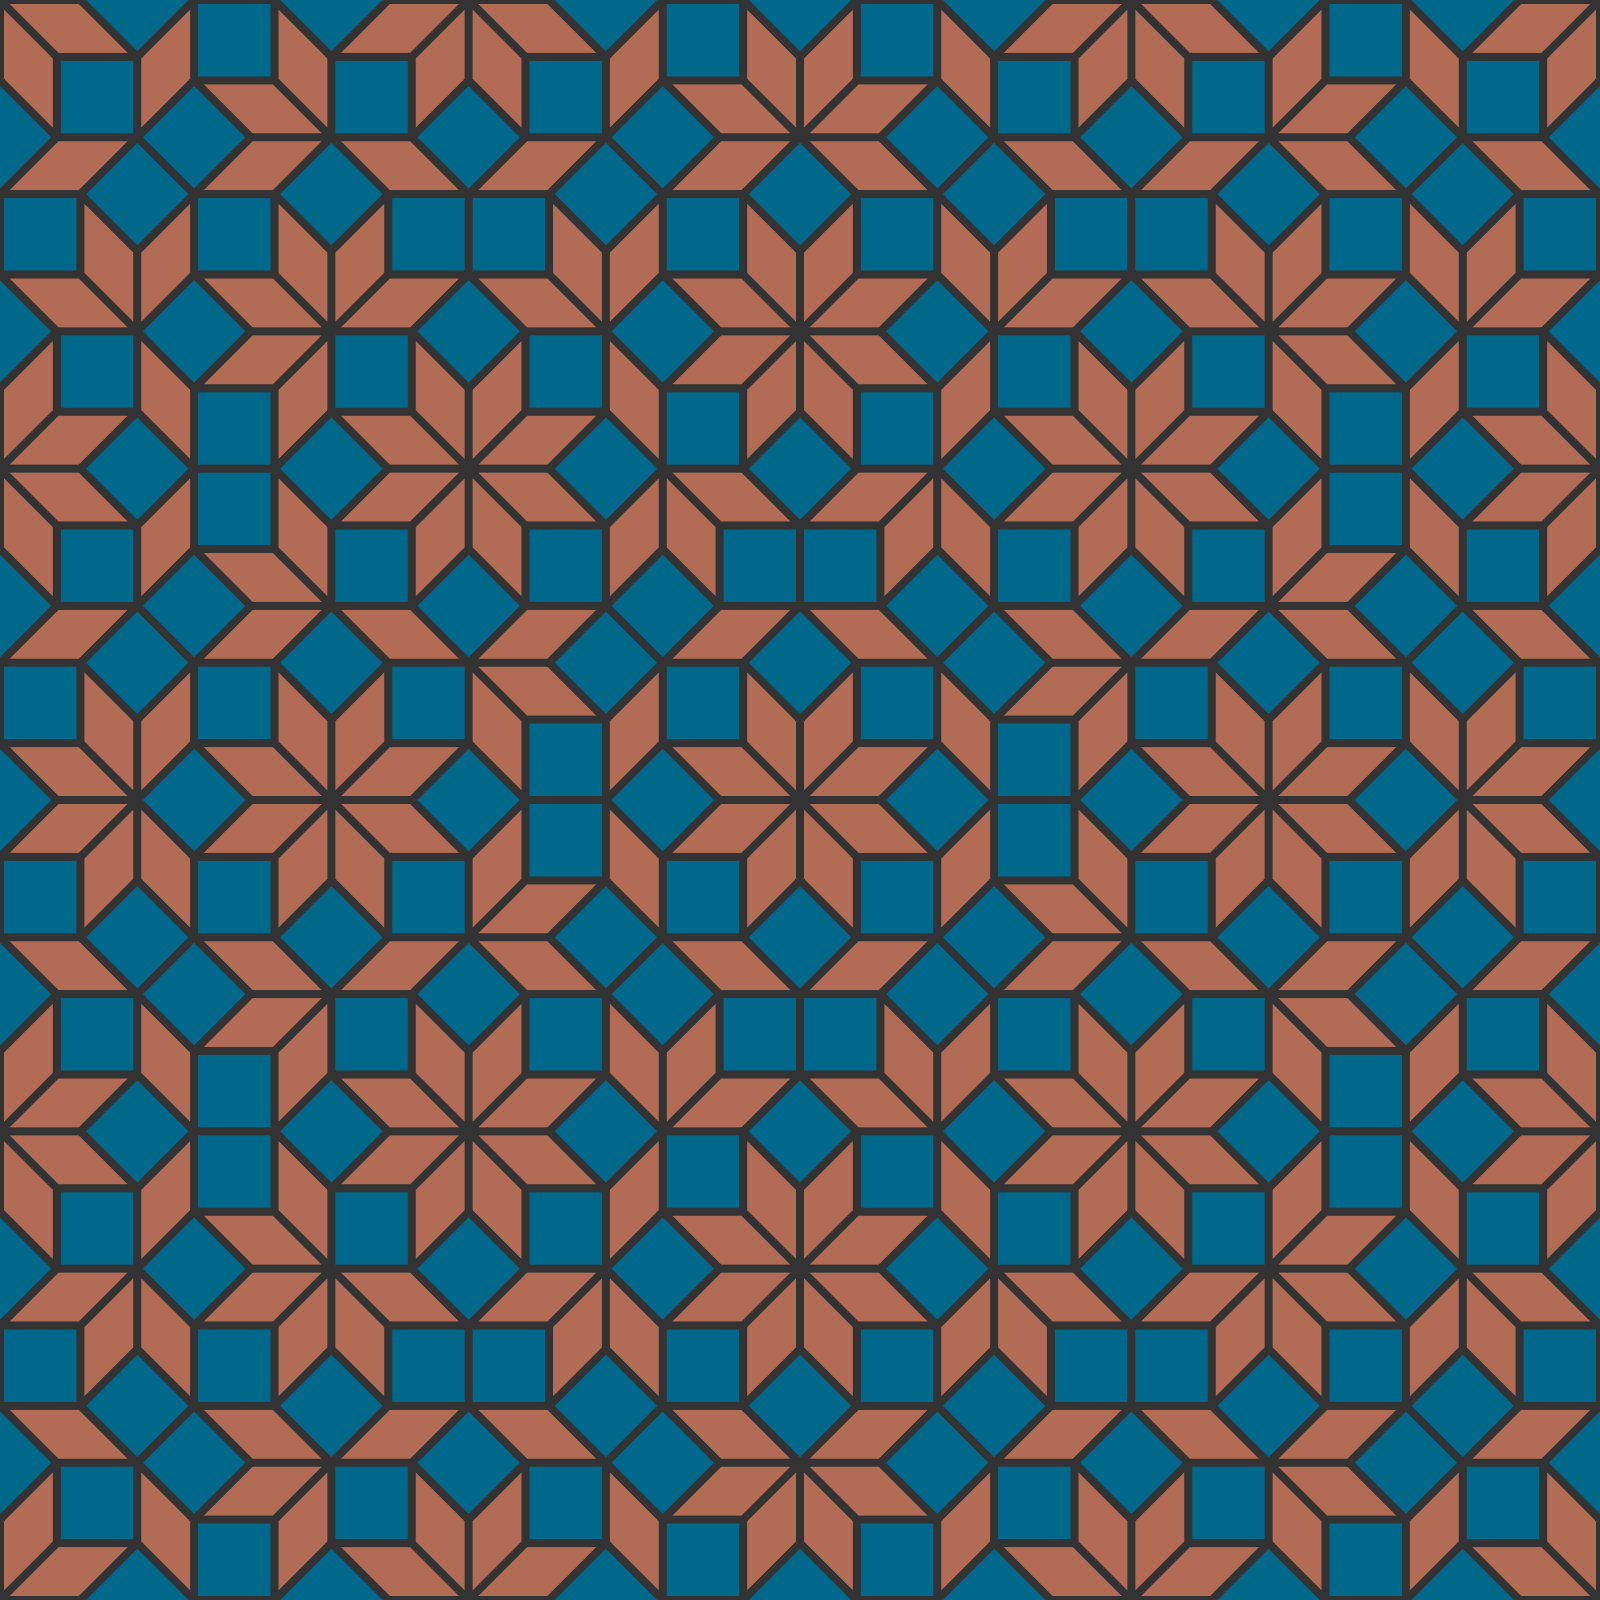
\includegraphics[scale=.08]{img/ammann-beenker.png}

}
\end{column}
\begin{column}{5cm}
{\centering
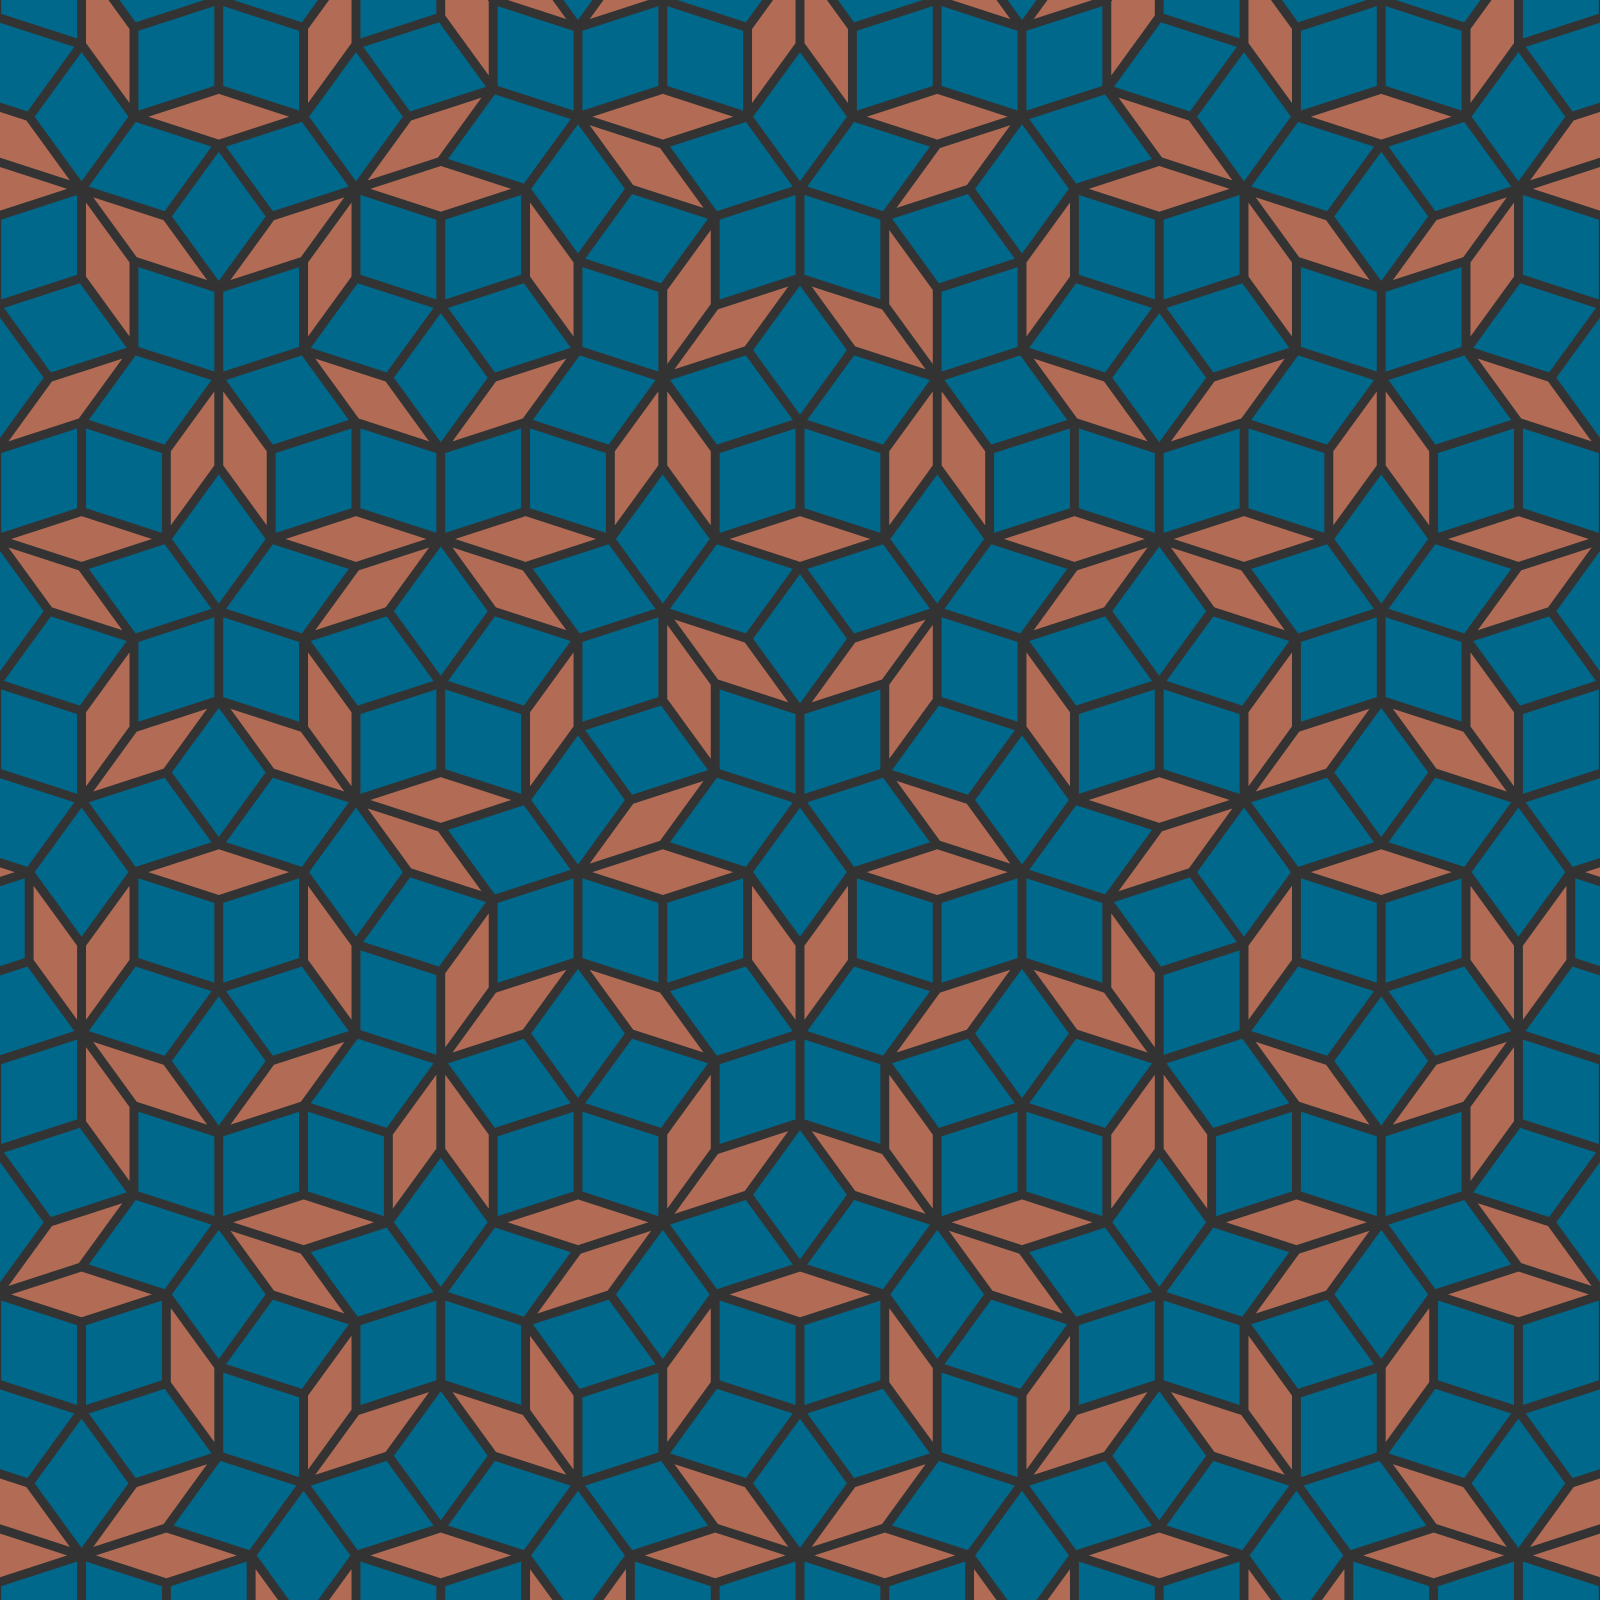
\includegraphics[scale=.08]{img/penrose.png}

}
\end{column}
\end{columns}
Model:
\[
	E \psi_m = V_m \psi_m + t\sum_{n \in V(m)} \psi_n
\]
The quasiperiodic features are encoded in the adjacency of the vertices.
\end{frame}

\begin{frame}{What is known}

Local density of states [taken from Zijlstra 2014]:

{\centering
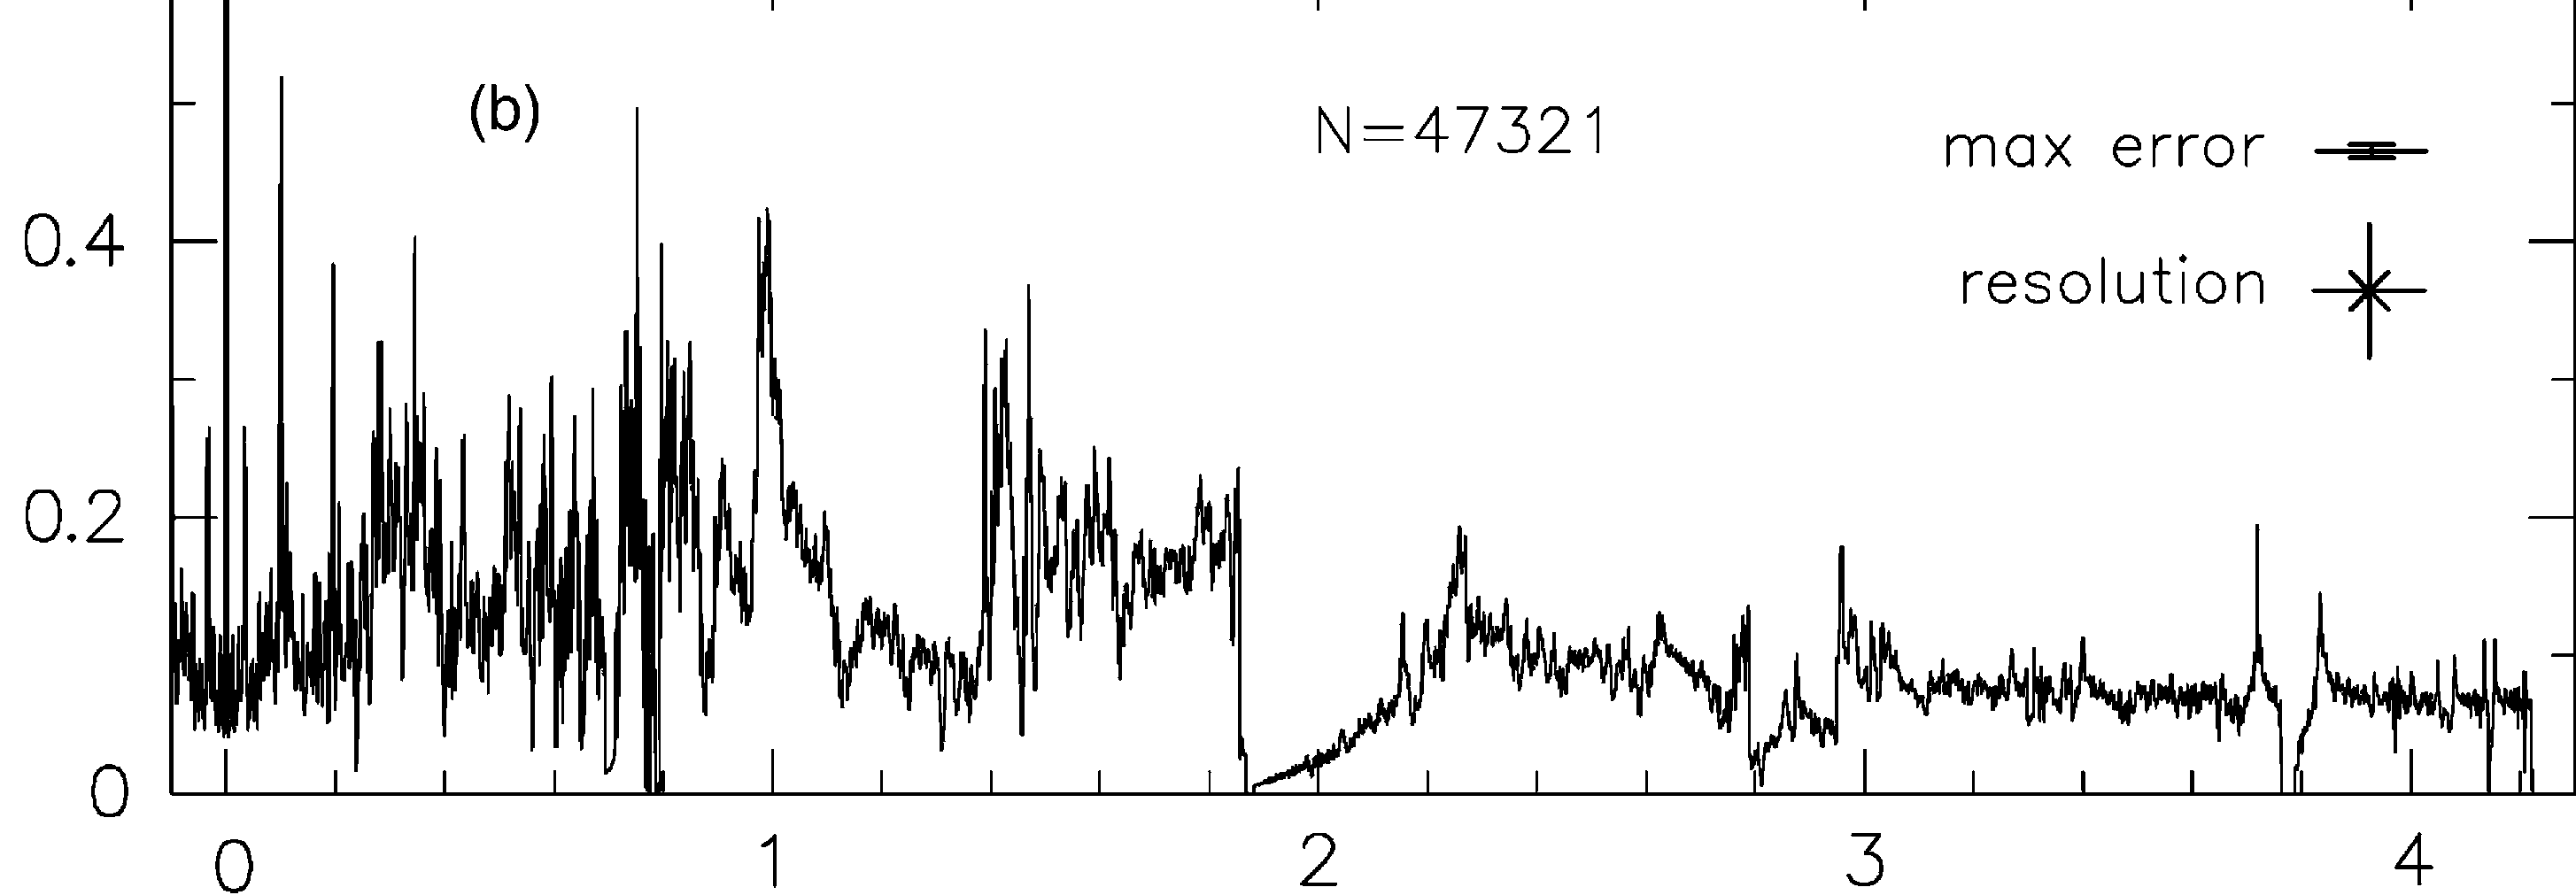
\includegraphics[scale=.1]{img/idos_AB_small.png}

}
\begin{itemize}
	\item Spectrum: no apparent fractal structure
	\item States are critical (numerical result, eg [Rieth, Schreiber 1998])
\end{itemize}
$\rightarrow$ can we introduce a field of arrows to describe some of these critical wavefunctions?
\end{frame}

\begin{frame}{A natural field of arrows}

In superspace, arrows go from the center to the border of the slice:

{\centering
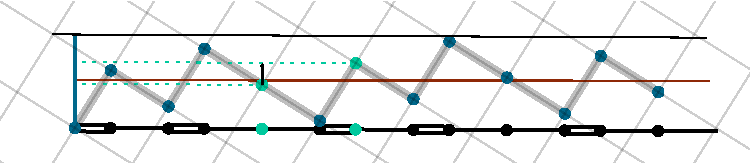
\includegraphics[scale=.8]{img/cut_and_project_arrows.pdf}

}

Define arrows in the same way for 2D tilings:

{\centering
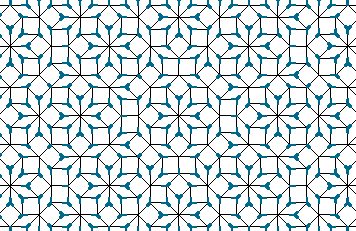
\includegraphics[scale=.9]{img/arrowed_tiling_excerpt.pdf}

}

State built with this arrow field? $\psi_m = \beta^{h(m)}$
\end{frame}

\begin{frame}{The groundstate wavefunction}
Can we find a state
\[
\psi_m = \beta^{h(m)} ?
\]
Idea [Sutherland 1986]: tune the potential
\[
	E \psi_m = V_m \psi_m + t \sum_{n \in V(m)} \psi_n \Longleftrightarrow V_m = E - t\sum_n \beta^{A_{m,n}}
\]
Not very physical! Generically, potential is detuned.

[Kalugin, Katz 2014] conjecture: state keeps its structure, but acquires a local modulation:
\[
	\psi_m = C_{m} \beta^{h(m)}
\]
where $C_m$ is local:
\[
	C_m \simeq C_n \text{~ if the environments around $m$ and $n$ agree on large distance }
\]
\end{frame}

\begin{frame}{Robustness of the structure}

\begin{columns}
\<{8cm}
\includegraphics[scale=.5]{img/gs.png}
\>
\<{4cm}
The groundstate is \textbf{very robust}: 
\[
	E \psi_m = V_m \psi_m + t\sum_{n} \psi_n
\]
for any $t$, $V_m$
\[
	\implies \psi_m = C_m \beta^{h(m)}
\]
(no proof, numerical results)
\>
\end{columns}
\end{frame}

\begin{frame}{Scaling analysis of the groundstate}

\begin{columns}
\<{7cm}
\begin{itemize}
	\item Participation ratio over a region $\mathcal{R}$:
	\[
		\text{PR}(\psi, \mathcal{R}) = \frac{\left( \sum_{m \in \mathcal{R}}|\psi_m|^2 \right)^2}{\left( \sum_{m\in \mathcal{R}} |\psi_m|^4 \right)^4}
	\]
	\item Scaling with the region volume $\text{Vol}(\mathcal{R})$:
	\[
		\text{PR}(\psi, \mathcal{R}) \sim \text{Vol}(\mathcal{R})^{D(\psi)}
	\]
	\begin{itemize}
		\item $D(\psi) = 0 \implies \psi$ localized
		\item $D(\psi) = 1 \implies \psi$ extended
		\item $0 < D(\psi) < 1 \implies \psi$ critical
 	\end{itemize}
\end{itemize}
\>

\<{7cm}
Assuming the form $\psi_m = C_m \rho^{h(m)}$ we can compute the scaling analytically:
\[
D(\psi) = \log\left( \frac{\omega(\rho^2)^2}{\omega(\rho^4)}\right)/\log \omega(1)
\]
with 
\begin{align*}
\omega(z) &= \frac{a(z)+\sqrt{a(z)^2 - z^2}}{z} \\
a(z) &= 4 z^2 + 9 z + 4
\end{align*}
\>
\end{columns}
\end{frame}

\begin{frame}{Conclusion}
\begin{itemize}
	\item Non-interacting eigenstates on quasicrystals are generically critical: here we were able to understand it for some specific states, both in 1D and 2D.
	\item On our examples, wavefunction construction involves a geometrical quasiperiodic function, the field of arrows.
	\item Its integral, the height function, has logarithmic growth,
	\item As a result, the wavefunction is critical: it has a local power law behavior.
\end{itemize}
Perspectives:
\begin{itemize}
	\item What happens for the grounstate of other quasicrystals, like the dodecagonal ones?
	\item For Penrose and AB, the arrow field cannot be used to describe other states. What extra ingredients are required?
\end{itemize}
\end{frame}

\begin{frame}{More perpsectives!}
\begin{itemize}
	\item A plot of the state just below the gap, with its quasiperiodic array of lines of zeros, that remain to be understood!
\end{itemize}
\end{frame}

%%%%%%%%%%%% Extra slides %%%%%%%%%%%%%
\begin{frame}{Cut and project chains are special!}
Consider the chain constructed by the substitution
\begin{align*}
	A & \to ABBB \\
	B & \to A
\end{align*}
\begin{columns}
\<{6cm}
\begin{itemize}
	\item This substitution cannot be built by cut and project (because it is non-Pisot).
	\item Height resembles a random walk, and typical height $\sim \sqrt{L}$
	\item As a result, the wavefunction is localized! 
\end{itemize}
\>
\<{6cm}
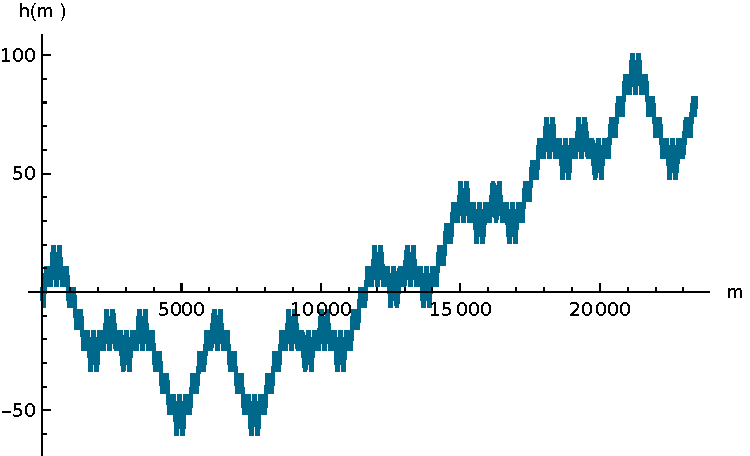
\includegraphics[scale=.5]{img/heightsB3.pdf}
\>
\end{columns}
$\rightarrow$ criticality is sensitive to the \textbf{complexity} of the tiling
\end{frame}



\end{document}